\documentclass[a4paper,11pt]{article}
\usepackage[margin=2cm]{geometry}

\usepackage[nodayofweek]{datetime}
\usepackage{cite}
\usepackage{graphicx}
\longdate

\usepackage{fancyhdr}
\pagestyle{fancyplain}
\fancyhf{}
\lhead{\fancyplain{}{M.Sc.\ Group Project Report}}
\rhead{\fancyplain{}{\today}}
\cfoot{\fancyplain{}{\thepage}}


\title{Implementation of attentional bistability of the dragonfly visual neurons in an intelligent biomimetic agent\\\Large{--- Report One ---}}
\author{Juan Carlos Farah, Panos Almpouras, Ioannis Kasidakis, Erik Grabljevec, Christos Kaplanis\\
       \{jcf214, pa512, ik311, eg1114, ck2714\}@doc.ic.ac.uk\\ \\
       \small{Supervisors: Professor Murray Shanahan, Zafeirios Fountas, Pedro Mart\'{i}nez-Mediano}\\
       \small{Course: CO530/533, Imperial College London}
}

\begin{document}
\maketitle

\section{Introduction}

Our goal in this project is to model the target selection mechanism of the dragonfly and implement it in a biomimetic agent. Dragonflies are notoriously effective at prey capture, making the neural processes that underlie this ability particularly interesting to investigate. 

The centrifugal small �target motion detector neuron 1 (CSTMD1) is a higher �order visual neuron in the brain of the dragonfly. This neuron reacts to the presentation of multiple visual stimuli by firing as if only one of the stimuli was present; this is presumably an attentional selection mechanism \cite{w13}. At Professor Shanahan's lab, they have simulated the large contralateral dendritic field of the CSTMD1 neuron with a biophysical multi­compartmental Hodgkin-Huxley model. Along with Klaus Stiefel \cite{ne13}, researchers found that with certain numbers of inhibitory synapses and potassium conductance densities, two mutually coupled CSTMD1 neurons are capable of a bistable switching process between two input patterns. This bistability can serve as a mechanism for the observed attentional selection.

The high­ level idea of the project is to employ the principle used by the CSTMD1 neuron in a biomimetic agent that behaves like a dragonfly, showing attention-�like target selection when performing a simple foraging task.

\section{Specification}
We brainstormed using goal-oriented capture in order to determine the requirements for our project. Below is a chart that portrays this process.	
		
	
	\begin{figure}
	\begin{center}
	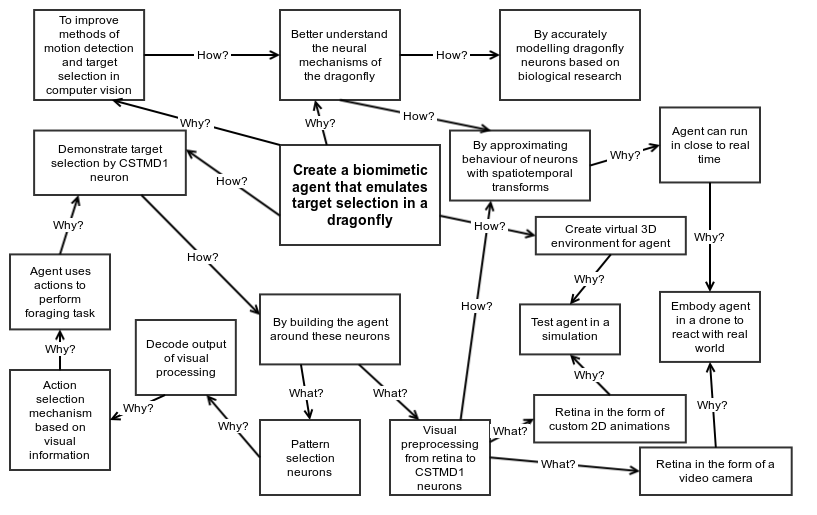
\includegraphics[scale = 0.5]{goalorient}
	\end{center}
	\end{figure}	
	

	\subsection{Minimum Requirements (Stage 1)}
	
	The goal-oriented capture enabled us to establish some minimum requirements for the completion of the project. In order to build an agent that can interact with its environment and exhibit the selective function of the CSTMD1 neuron, three main objectives need to be completed:
\begin{enumerate}
	\item (1A) We need to connect the visual input of the agent (in the form of either a camera input or a constructed animation) to the modelled CSTMD1 neurons. This will involve:
	\begin{enumerate}
		\item Building a model of the visual processing that occurs between the retina and the actual CSTMD1 neurons of a real dragonfly.
		\item Deciding how many CSTMD1 neurons we will use and how exactly to connect them to the output of our visual pre-processing.
		\item Once connected, test the system for various inputs from simple animations to see if we can recreate the selectivity between two targets observed in actual CSTMD1 neurons \cite{w13}.
	\end{enumerate}
	\item (1B) We need to build a layer of pattern recognition neurons that can decode the output of the CSTMD1 neurons.
	\item (1C) We need to integrate the visual processing and the pattern recognition system and add a simple action selection mechanism. For the minimum requirement, we will need two neurons that take input from the pattern recognition system that fire when the dragonfly chooses to go left or right respectively to catch a target.
\end{enumerate} 
 
 	\subsection{Expected implementation (Stage 2)}
 	
 	Beyond the minimum requirements, we expect to enhance the action selection mechanism in order to give a more complex reaction to targets in the visual field . This will involve:
 \begin{enumerate}
 	\item Creating a virtual 3D environment for the dragonfly agent.
 	\item Enhancing the action-selection mechanism to have at least 12 output neurons, giving the dragonfly six degrees of freedom (three for rotation and three for translation).
 	\item Employing reinforcement learning in the action selection mechanism to train the agent to move more effectively towards the target.
 \end{enumerate}
 
 	\subsection{Possible extensions (Stage 3)}
 	
 	Beyond the expected implementation, these are ways we have thought of to extend the project:
 \begin{enumerate}
 	\item Implement the agent in a quadcopter drone (owned by the Neurodynamics Lab).
 	\item Replace normal camera with an event-based camera to more realistically emulate the dragonfly retina.
 	\item Improve user interface of virtual simulation environment (allow user to change number and speed of targets, etc.). 
 \end{enumerate}

\section{Development Methodology}

\subsection{Project Management}

\subsubsection{Agile Scrum}

Given the complexity of our project and its division into clear working stages, we chose to apply the Scrum Methodology of Agile Development as our project management framework.

\subsubsection{Sprints}
The project has been divided into seven two-week sprints starting on 4 February 2015. The first five sprints have been designed to complete the minimum and expected goals, with the last two reserved to refine results, prepare the presentation and optionally implement extensions. Sprint Review meetings will be held every other Wednesday in the presence of co-supervisors Zafeirios Fountas and Pedro Mart\'{i}nez, followed directly by the Sprint Planning meeting for the upcoming sprint. Sprints are being managed using Trello, with each task given an estimate of one to eight hours and a priority ranging from one (highest) to three (lowest).

\subsubsection{Stand-Ups}
Every weekday the team meets for a brief stand up meeting capped at 15 minutes. During this time, the state of the current sprint is assessed, with each team member outlining what he achieved on the previous day and what he will be working on before the next stand-up. Any possible bottlenecks or roadblocks identified during these stand-ups are later addressed by the Team Leader.

\subsection{Collaboration Tools}

\subsubsection{Communication Channels}
All of our communication is conducted using Slack, which allows team members visibility to all aspects of the project. Relevant information is shared, discussed and classified using Slack's channeled feeds, with a dedicated channel assigned to each sprint.

\subsubsection{Version Control}
We are using Git as our version control system, hosting our remote repository on GitLab, which integrates with our communication and project management tools. By taking advantage of web hooks, pushes to the repository can trigger automatic code reviews and unit tests, ensuring code integrity and keeping all team members and supervisors up to date with progress.

\section{Task scheduling}
\subsection{Stage 1A: Visual Pre-processing}
\begin{center}
    \begin{tabular}{p{12cm} c c}
    \textbf{Task} & \textbf{Priority} & \textbf{Sprint} \\ \hline
	Implement visual pre-processing chain based on \cite{hal11}. & 1 & 1 \\
	Connect output of pre-processing to CSTMD1. & 1 & 1\\
	Replicate experiment in \cite{w13}. & 1 & 1 \\
    \end{tabular}
\end{center}

\subsection{Stage 1B: Pattern Recognition}
\begin{center}
    \begin{tabular}{p{12cm} c c}
    \textbf{Task} & \textbf{Priority} & \textbf{Sprint} \\ \hline
	Consolidate Spike-Response Model neuron as a Python class. & 2 & 1 \\
	Consolidate pattern and noise sample generators as a Python class. & 2 & 1 \\
	Design and implement unit tests for neuron model. & 2 & 1 \\
	Design and implement unit tests for generators. & 2 & 1 \\
	Add the ability to save and load samples for testing. & 3 & 1 \\
	Make single pattern recognition neuron into a module. & 1 & 1 \\
	Extend single pattern recognition neuron to a model of competing patterns. & 1 & 1 \\
	Analyse impact of varying noise on pattern recognition neurons. & 2 & 1 \\
    \end{tabular}
\end{center}

\subsection{Stage 1C: Integration and Basic Action Selection}
\begin{center}
    \begin{tabular}{p{12cm} c c}
    \textbf{Task} & \textbf{Priority} & \textbf{Sprint} \\ \hline
	Define the points of integration between both modules. & 1 & 2 \\
	Design unit tests for connecting neurons. & 1 & 2 \\    
	Connect visual pre-processing neurons to pattern recognition neurons. & 1 & 2 \\
	Implement two action selection neurons. & 1 & 2\\
	Train action selection neurons with reinforcement learning. & 1 & 2\\    
	Implement unit tests for sample visual input. & 2 & 2 \\
    \end{tabular}
\end{center}

\subsection{Stage 2: Enhanced Action Selection Mechanism}
\begin{center}
    \begin{tabular}{p{12cm} c c}
    \textbf{Task} & \textbf{Priority} & \textbf{Sprint} \\ \hline
	Define range of actions available to the biomimetic agent. & 1 & 3 \\
	Create tests to measure success of action taken given input. & 1 & 3 \\ 
	Design basic environment for simulated agent. & 1 & 3 \\
	Implement basic environment for simulated agent. & 1 & 4 \\
	Implement unit tests to ensure integrity with rest of the system. & 2 & 4 \\
	Extend simulated environment to approach behaviour in nature. & 3 & 4 \\
	Run extended tests with various inputs and refine mechanism. & 2 & 5 \\
	Analyse how results compare to the literature. & 2 & 5 \\
    \end{tabular}
\end{center}

\subsection{Stage 3: Embodiment of Agent for Real-World Interaction}
\begin{center}
    \begin{tabular}{p{12cm} c c}
    \textbf{Task} & \textbf{Priority} & \textbf{Sprint} \\ \hline
	Prepare software in agent for prototyping. & 3 & 6 \\
	Set wireless real-time connection between GPU and agent. & 3 & 6 \\
	Define measure of success for agent's interaction with its environment. & 3 & 6 \\
	Write unit tests for sample simulations in agent's operating system. & 3 & 6 \\
	Test agent in predefined real-world environment. & 3 & 7 \\
	Analyse effect of different targets on success of agent. & 3 & 7 \\
    \end{tabular}
\end{center}	

%%%%%%%%%%%%%%%%%%%%%%%%%%%%%%%%%%%%%%%%%%%%%%%%%%%%%%%%%%%%

\section{Work Allocation}

\subsection{Organisation}

Juan Carlos Farah was selected to become Group Leader, due his experience in organisation and software development. He took responsibility for project coordination and code integration. Our project is split in three stages and we are allocating team members to tasks on a rolling basis. For stage one we have split the team into two sub-groups. One sub-group is working on visual pre-processing, while the other is working on pattern recognition. We assign members according to an estimation of how long each part will take. The table below shows how we have allocated work so far:

\begin{table}[ht]

\centering % used for centering table

\begin{tabular}{l c c c c c} % centered columns (4 columns)

%inserts double horizontal lines

& Leader & Stage 1A & Stage 1B & Stage 2 & Stage 3\\ [0.5ex] % inserts table

%heading

\hline % inserts single horizontal line

Juan Carlos Farah & x & & x & x & x \\ % inserting body of the table

Erik Grabljevec & & x & & x & x \\

Christos Kaplanis & & x & & x & x \\

Panagiotis Almpouras & & & x & x & x \\

Ioannis Kasidakis & & x & & x & x \\ [1ex] % [1ex] adds vertical space

\end{tabular}

\label{table:nonlin} % is used to refer this table in the text

\end{table}

%%%%%%%%%%%%%%%%%%%%%%%%%%%%%%%%%%%%%%%%%%%%%%%%%%%%%%%%%%%%

\section{Feasibility and Risks}

Each of the components of our minimum and expected requirements is being structured according to relevant published research that serves as its starting point and general heuristic. This allows us to outline the aforementioned specifications so that the core of our project is highly feasible from the onset. Stage 1A bases itself on \cite{hal11}, Stage 1B on \cite{stdp1} and \cite{stdp2}. Moreover, our approach for Stage 2 will stem from \cite{tsdn}.

Nevertheless, there are a number of risks that could influence the outcome of our project. Firstly, it is important to highlight that our team is not fully acquainted with a number of computational neurodynamics concepts. Secondly, following modular development, each of the components our project is being developed independently. This introduces the possibility of incompatibility between each of the parts. This is exemplified by the complex connections needed between the visual pre-processing, CSTMD1 and pattern recognition neurons, and furthermore, between these and the action-selection mechanism. We are continually addressing these respective risks by going through recommended readings provided by our supervisors and maximising communication channels, code integrity and visibility as specified in our project methodology.

\section{Project Boundaries}

\subsection{Software}
Software development will be predominantly done using Python. The numpy library is particularly useful for the purposes of this project as, among other features, it provides functions for fast matrix manipulations. To appropriately process the visual input (from the camera), we will use OpenCV for spatial transforms and the scipy library for temporal filters. This way we can discard irrelevant information before the frames of the input are sent for processing. The CSTMD1 neuron is modelled using NEURON, a simulation environment created by Yale University, which has the power to very accurately model individual neurons. We are learning to use this library in order to connect the CSTMD1s to our other neurons.

\subsection{Hardware}
Having the agent running in close to real-time will require significant computer processing power. Although prototyping will be done using the virtual machine we were provided, staging and testing will be undertaken using the GPU-accelerated computer located in the Neurodynamics Lab. To make an actual drone behave like a dragonfly, it will have to be equipped with a camera. The input signal will be sent to the GPU for processing which in turn would send back instructions to the drone with the required movement it has to make. This constant exchange of information between the drone and the remote GPU is highly likely to create delay in the response of the drone to the movement of the target. Thus, this is one of the limitations of this project. A more accurate realistic application would require a light weight and at the same powerful GPU to be installed on the drone so that all required computations can be done locally. 

\subsection{Audience}
This project is mostly relevant to academic research in the field of Computational Neuroscience. The ultimate goal is to publish an academic paper based on this project.


\bibliography{report1}{}
\bibliographystyle{plain}

\end{document}

